% Phase 2 project report, IEEE conference format.  Build:  cd project_report_phase2 && tectonic project_report.tex
\documentclass[conference]{IEEEtran}
\usepackage{iftex}
\ifPDFTeX
  \usepackage[T1]{fontenc}
\else  % XeLaTeX / Tectonic: Times-compatible OpenType font
  \usepackage{fontspec}
  \setmainfont{texgyretermes}[Extension=.otf, UprightFont=*-regular, BoldFont=*-bold,
    ItalicFont=*-italic, BoldItalicFont=*-bolditalic]
\fi
\usepackage{amsmath,amssymb}
\usepackage{graphicx}
\usepackage{booktabs}
\usepackage{tikz}
\usetikzlibrary{positioning,arrows.meta,fit}
\usepackage[hidelinks]{hyperref}
\usepackage{cite}
\graphicspath{{../results/figures/}}
\tikzset{
  box/.style={draw=black!70, rounded corners=2pt, fill=white, minimum height=2.2em, align=center, font=\small, inner sep=4pt},
  dl/.style={box, draw=blue!60!black, fill=blue!6},
  ml/.style={box, draw=orange!80!black, fill=orange!8},
  arr/.style={-{Stealth[length=2mm]}, thick, black!70},
}
% start a second row of author blocks
\makeatletter
\newcommand{\linebreakand}{\end{@IEEEauthorhalign}\hfill\mbox{}\par\mbox{}\hfill\begin{@IEEEauthorhalign}}
\makeatother

\begin{document}

\title{Traffic Flow Prediction on METR-LA with Graph Attention Networks and a Hybrid Model}

\author{
\IEEEauthorblockN{Deepanshu}\IEEEauthorblockA{Enrollment No. 2401010144}
\and
\IEEEauthorblockN{Kanishk Sharma}\IEEEauthorblockA{Enrollment No. 2401010207}
\and
\IEEEauthorblockN{Adarsh}\IEEEauthorblockA{Enrollment No. 2401010026}
\linebreakand
\IEEEauthorblockN{Daksh Yadav}\IEEEauthorblockA{Enrollment No. 2401010139}
\and
\IEEEauthorblockN{Hrishabh Prajapati}\IEEEauthorblockA{Enrollment No. 2401020027}
}

\maketitle

\begin{abstract}
We forecast traffic speed 5 to 60 minutes ahead at the 207 sensors of the METR-LA dataset
and ask whether a model that uses the road network does better than separate models for
each road segment. We trained three models. The first is a set of 207 XGBoost models, one
per sensor, that only see their own sensor's history (MAE 3.20\,mph). The second, ST-GAT,
is a graph attention network that lets every sensor look at its upstream and downstream
neighbours on the road graph (3.04\,mph). The third is a hybrid in which the graph network
learns a correction to the XGBoost forecasts (3.06\,mph, and the best model at 15 minutes).
Both network models beat the per-segment models at every horizon, with the largest gains
during rush hour and congestion. Ablation runs show that most of the gain comes from using
the road graph and from handling missing sensor readings properly. A simple offline
experiment also shows that the better forecasts would let a traffic signal switch to a
congestion plan earlier. This is a simulation only; we did not control real signals.
\end{abstract}

\begin{IEEEkeywords}
traffic forecasting, graph attention networks, spatio-temporal deep learning, hybrid models,
XGBoost, METR-LA
\end{IEEEkeywords}

% ---------------------------------------------------------------- 1
\section{Introduction}
Short-term traffic forecasts are used for route guidance, ramp metering and choosing signal
plans. A common way to build them is to train one model for each road segment using only
that segment's past readings. These models are easy to train and maintain, but they cannot
see what is happening on nearby roads. When a queue forms at the next interchange, the
segment behind it will slow down a few minutes later, and a model that only looks at its own
segment has no way of knowing this in advance.

The question of this project is whether a model that learns over the whole road network
predicts better than independent segment models, and in which situations. We compare three
models on the METR-LA benchmark~\cite{li2018dcrnn}:
\begin{enumerate}
\item \textbf{XGBoost per segment:} 207 separate gradient-boosting models, one per sensor.
\item \textbf{ST-GAT:} a spatio-temporal graph attention network over the road graph.
\item \textbf{Hybrid:} the XGBoost forecasts corrected by a graph attention network.
\end{enumerate}
All three are trained and tested on the same data with the same one-hour input window. We
report MAE, RMSE and MAPE at every horizon, separately for peak and off-peak hours, test the
differences statistically, and run ablations to see which parts of each model matter.

% ---------------------------------------------------------------- related work
\section{Related Work}
Early traffic forecasting used statistical time-series models such as ARIMA~\cite{ahmed1979},
which work on one sensor at a time and lose accuracy quickly at longer horizons. Tree ensembles
such as gradient boosting and XGBoost~\cite{chen2016xgboost} handle non-linear patterns well and
are still strong per-segment baselines, but they depend on hand-made features. Recurrent
networks such as LSTMs~\cite{hochreiter1997} learn from the raw series, yet they also treat each
sensor separately.

Graph neural networks were introduced to use the road network. DCRNN~\cite{li2018dcrnn} models
traffic as diffusion on the directed road graph inside a recurrent encoder--decoder and released
the METR-LA dataset. STGCN~\cite{yu2018stgcn} alternates temporal convolutions with graph
convolutions, Graph WaveNet~\cite{wu2019gwnet} learns an extra adjacency matrix, and
GMAN~\cite{zheng2020gman} builds the whole model from attention. Graph attention
networks~\cite{velickovic2018gat} let each node learn how much weight to give to each neighbour,
and ASTGCN~\cite{guo2019astgcn} applies attention to traffic. Our ST-GAT follows the block design
of STGCN but uses graph attention on the fixed road graph, with separate attention to upstream
and downstream sensors.

Combining a classical model with a neural network is an older idea: Zhang~\cite{zhang2003hybrid}
fits a neural network to the errors of an ARIMA model, and stacking~\cite{wolpert1992stacking}
trains a second model on out-of-sample predictions of the first. Our hybrid uses the same idea
with XGBoost and graph attention. For missing values we follow GRU-D~\cite{che2018grud}, which
showed that an explicit missing-value mask helps neural networks. Signal-control studies usually
need a traffic simulator such as SUMO~\cite{krajzewicz2012sumo} or
CityFlow~\cite{zhang2019cityflow}; since METR-LA has no signal data, we only run an offline
replay.

% ---------------------------------------------------------------- 2
\section{Dataset and Experimental Setup}
\subsection{METR-LA}
METR-LA~\cite{li2018dcrnn} contains speed readings from 207 loop detectors on Los Angeles
freeways, recorded every 5 minutes from 1 March to 27 June 2012 (34,272 time steps). It also
gives the road distance between sensors. Only speed is available, so we could not use flow or
occupancy. About 8.1\,\% of the readings are missing and stored as 0\,mph, and there are 2,148
time steps where the whole network was down.

We build the adjacency matrix from the road distances with the Gaussian kernel used by
DCRNN~\cite{li2018dcrnn}:
\begin{equation}
W_{ij}=\begin{cases}\exp\!\left(-d_{ij}^2/\sigma^2\right) & \text{if this is at least } 0.1,\\ 0 & \text{otherwise,}\end{cases}
\end{equation}
where $d_{ij}$ is the road distance from sensor $i$ to sensor $j$ and $\sigma$ is the standard
deviation of all distances. The resulting graph has 1,515 directed edges, 73\,\% of them
one-way, and each sensor has on average 36 other sensors within two hops.

\subsection{Forecasting task and split}
Each sample uses the last 12 readings (one hour) of every sensor to predict the next 12
readings (5 to 60 minutes ahead). We split the samples by time, never randomly: the first
70\,\% for training (23,974 windows, 1 March to 23 May), the next 10\,\% for validation
(3,425 windows) and the last 20\,\% for testing (6,850 windows, 4 to 27 June). The test set was
used only once, after all choices had been made.

\subsection{Preprocessing}
A missing reading looks like a speed of 0\,mph, which a model could mistake for a complete
standstill. For the inputs we replace a missing reading with the last observed value and add
a 0/1 channel that says whether the reading was real. Missing target values are left out of
the loss and of all metrics. Speeds are standardised with the mean (58.58\,mph) and standard
deviation (12.83\,mph) of the training readings only. Time of day and day of week are encoded
as $\sin$ and $\cos$ pairs, so that 23:55 is close to 00:00.

\subsection{Metrics and tests}
We compute MAE, RMSE and MAPE on all observed test readings at every horizon. Peak hours are
weekdays 06:00--10:00 and 15:00--19:00, and a reading counts as congested if it is below
40\,mph. To check whether two models really differ, we use the Diebold--Mariano
test~\cite{diebold1995} with a Newey--West variance, which accounts for the overlap between
consecutive forecast windows.

% ---------------------------------------------------------------- 3
\section{Model 1: XGBoost per Segment}
\subsection{Features and model}
For each sensor we train one XGBoost~\cite{chen2016xgboost} model that only uses that
sensor's own data. Its 37 input features are the 12 most recent speeds, the change over the
last 5 and 15 minutes, the mean, standard deviation and minimum over the last hour, the
number of missing readings, time of day and day of week, and the sensor's usual speed for
that time of the week (computed from the training data) at each of the 12 target times.

Instead of one model per horizon we use XGBoost's multi-output trees, where every leaf stores
all 12 forecasts. On six random sensors this was slightly more accurate than one tree per
horizon (validation MAE 2.721 against 2.738\,mph). The models use the absolute-error loss,
trees of depth 6, a learning rate of 0.1 and up to 400 trees, with early stopping on the
validation data. Training all 207 sensors takes about 24 minutes on a laptop CPU.

\subsection{What the model learns}
Figure~\ref{fig:xgb} shows which features the trees use, averaged over 30 random sensors. More
than half of the gain comes from the sensor's usual speed at the target time (57\,\%) and about
a quarter from the recent speeds (24\,\%), with the latest reading being the most important
single feature. In other words, the model predicts the usual pattern for that time of week
and adjusts it with the current reading. Early stopping keeps a median of 113 trees per
sensor.

\begin{figure*}[t]
\centering
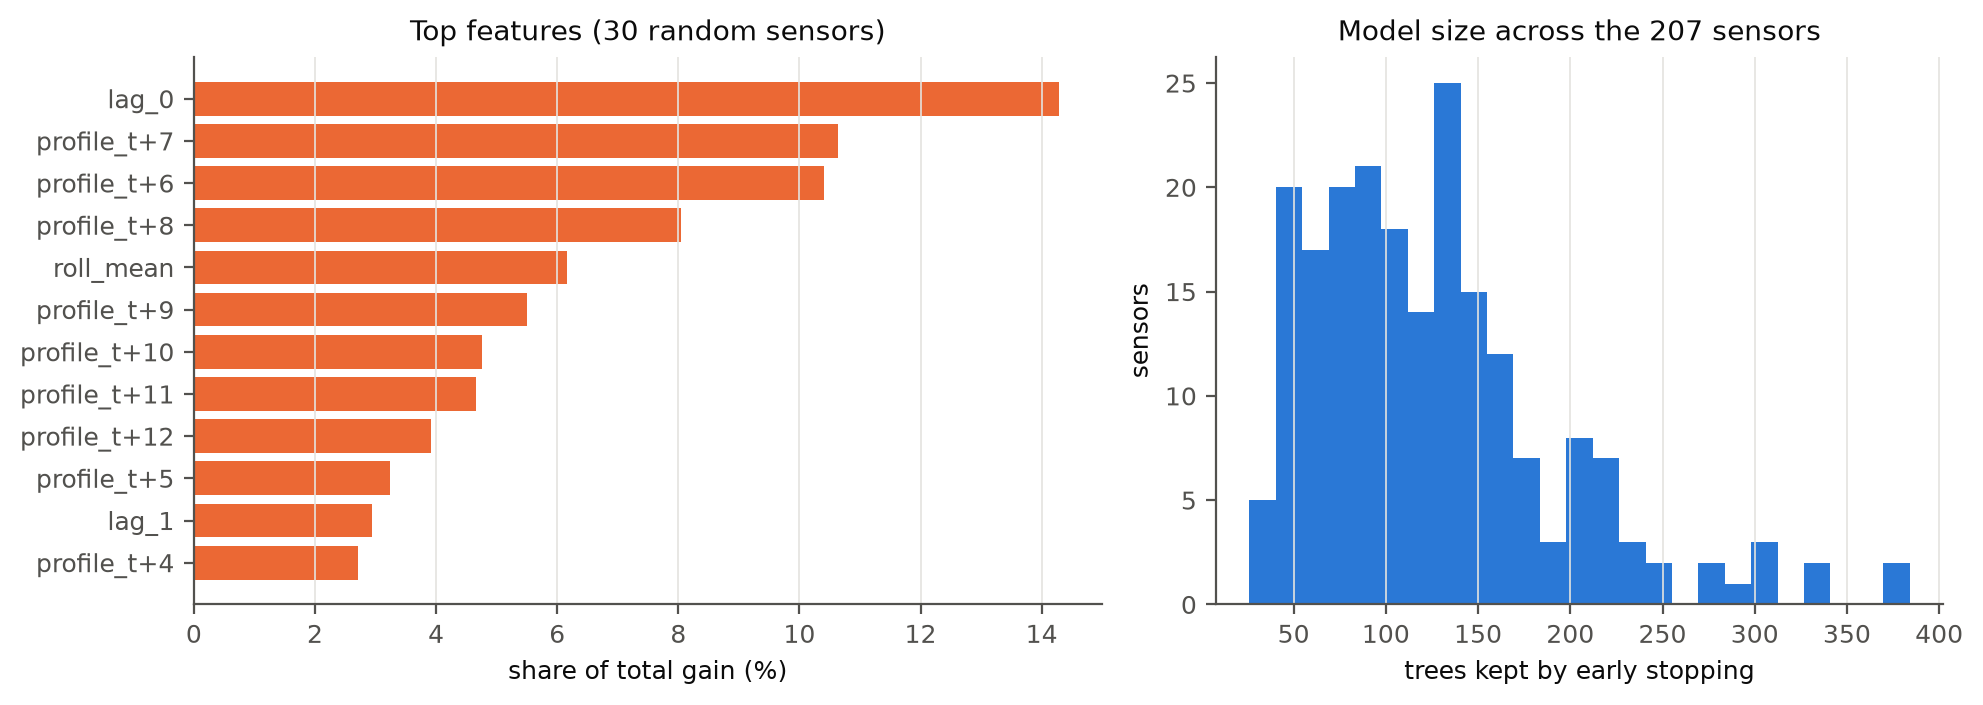
\includegraphics[width=\textwidth]{p2_xgb_importance.png}
\caption{XGBoost per segment. Left: the most important features (share of total gain, 30
sensors). Right: number of trees kept for each of the 207 sensors.}
\label{fig:xgb}
\end{figure*}

\subsection{What the model misses}
To see what an independent model cannot capture, we looked at its errors on the training
data. We used out-of-fold forecasts, so these errors are realistic and the test set is not
involved. Figure~\ref{fig:gap} shows two things. The errors of sensors that are close on the
road are correlated (0.21 at 60 minutes for neighbours against 0.04 for other pairs), and the
correlation falls with distance. The error is also more strongly related to the current state
of the downstream neighbours than to the sensor's own state, which the model already used.
This is information from other sensors that an independent model never sees. If the best
forecast that uses only sensor $i$ is $m_i$ and the best forecast using the whole network is
$m_{\mathcal{G}}$, then
\begin{equation}
\begin{split}
&\mathbb{E}\big[(y-m_i)^2\big]-\mathbb{E}\big[(y-m_{\mathcal{G}})^2\big]\\
&\qquad=\mathbb{E}\big[(m_{\mathcal{G}}-m_i)^2\big]\ \ge 0,
\end{split}
\end{equation}
so the network can only help, and it helps exactly when the per-segment errors depend on
other sensors, which is what we observe.

\begin{figure*}[t]
\centering
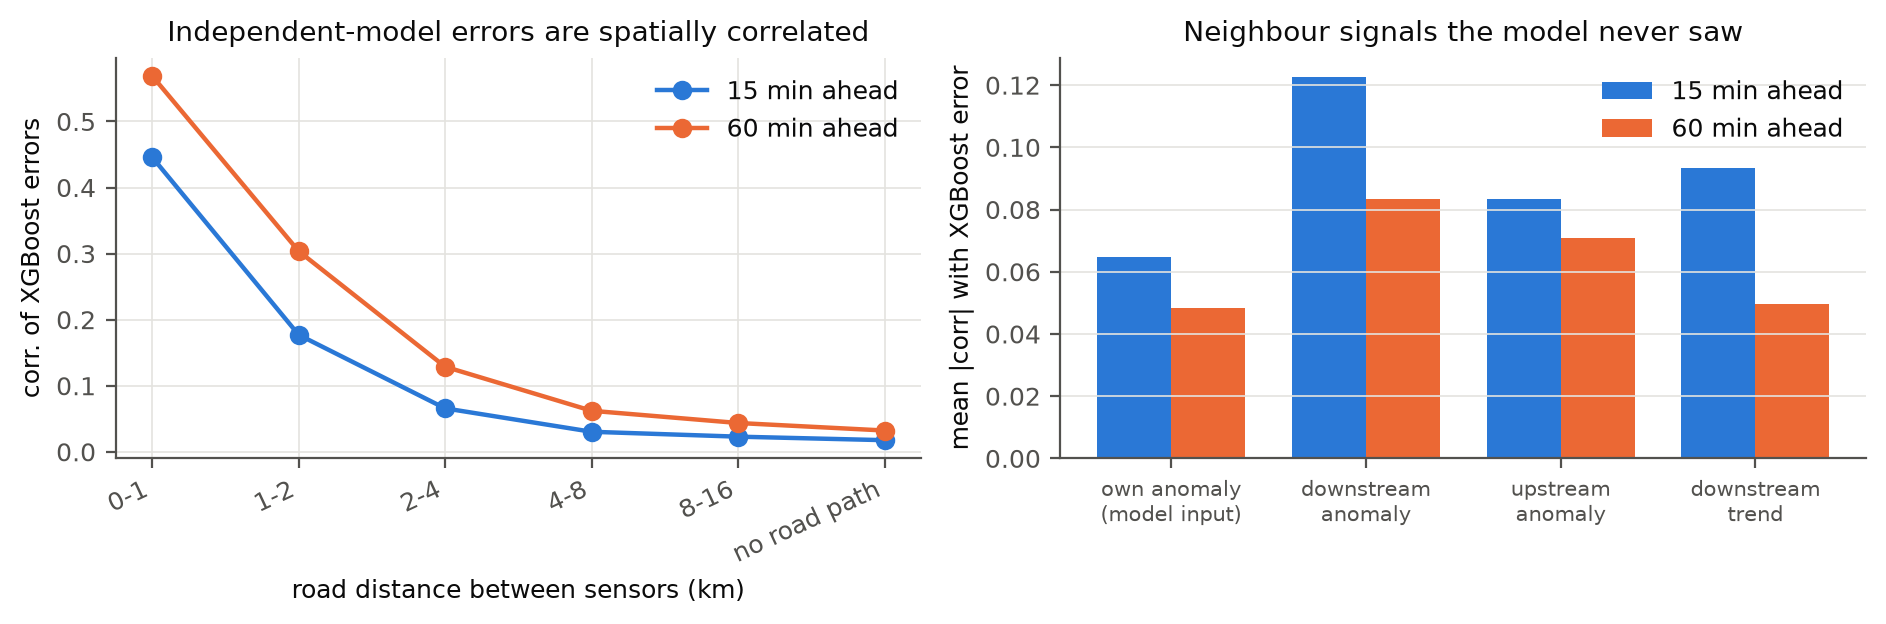
\includegraphics[width=\textwidth]{p2_gap_analysis.png}
\caption{Errors of the per-segment XGBoost models on out-of-fold training data. Left:
correlation of errors between sensor pairs by road distance. Right: correlation of the error
with information available at forecast time.}
\label{fig:gap}
\end{figure*}

% ---------------------------------------------------------------- 4
\section{Model 2: ST-GAT}
\subsection{Architecture}
ST-GAT forecasts all 207 sensors together. Its input is a $12\times207\times6$ window: the
filled-in speed, the 0/1 missing flag and four time features for every step and sensor. We
also give each sensor a learned 16-dimensional embedding so the model can learn
sensor-specific behaviour. A $1\times1$ convolution maps the inputs to 64 channels, then two
blocks process them (Fig.~\ref{fig:stgat}). Each block has a gated temporal convolution, a
graph attention layer and a second gated temporal convolution, followed by layer
normalisation and dropout, similar to the block design of STGCN~\cite{yu2018stgcn}. The
temporal convolutions have no padding, so the 12 time steps shrink to 10, 8, 6 and 4. A last
convolution reduces them to one vector per sensor, and a small fully connected network
outputs all 12 forecasts at once. The model has 163,516 parameters.

\begin{figure*}[t]
\centering
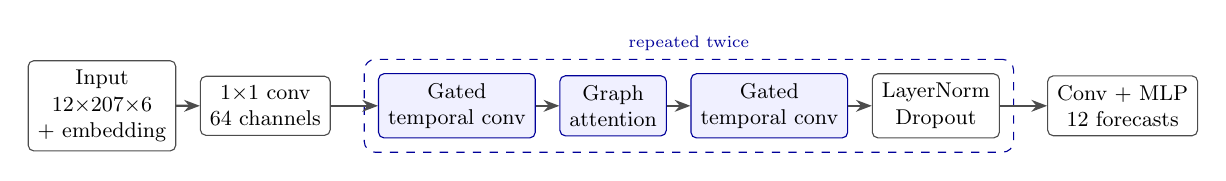
\begin{tikzpicture}[node distance=4mm and 3.5mm, scale=0.86, transform shape]
\node[box] (in) {Input\\$12{\times}207{\times}6$\\+ embedding};
\node[box, right=of in] (lift) {$1{\times}1$ conv\\64 channels};
\node[dl, right=7mm of lift] (t1) {Gated\\temporal conv};
\node[dl, right=of t1] (gat) {Graph\\attention};
\node[dl, right=of gat] (t2) {Gated\\temporal conv};
\node[box, right=of t2] (ln) {LayerNorm\\Dropout};
\node[draw=blue!60!black, dashed, rounded corners, fit=(t1)(gat)(t2)(ln), inner sep=5pt,
      label={[font=\scriptsize, text=blue!60!black]above:repeated twice}] {};
\node[box, right=7mm of ln] (out) {Conv + MLP\\12 forecasts};
\draw[arr] (in) -- (lift); \draw[arr] (lift) -- (t1); \draw[arr] (t1) -- (gat);
\draw[arr] (gat) -- (t2); \draw[arr] (t2) -- (ln); \draw[arr] (ln) -- (out);
\end{tikzpicture}
\caption{ST-GAT architecture.}
\label{fig:stgat}
\end{figure*}

\subsection{Gated temporal convolution}
The temporal convolution looks at 3 consecutive time steps and produces two sets of
channels, $P$ and $Q$. The output is
\begin{equation}
\Gamma(H)=\big(P+H\big)\odot\sigma(Q),
\end{equation}
where $H$ is the input (cropped to the right length) and the sigmoid of $Q$ works as a gate
that decides how much of each channel is passed on~\cite{dauphin2017glu}.

\subsection{Graph attention}
The graph attention layer follows Veli\v{c}kovi\'c et al.~\cite{velickovic2018gat}. For a sensor
$i$ and each neighbour $j$ on the road graph (including $i$ itself) it computes a score and
turns the scores into weights with a softmax:
\begin{gather}
s_{ij}=\mathrm{LeakyReLU}\big(\mathbf{a}_1^\top W h_i+\mathbf{a}_2^\top W h_j\big),\\
\alpha_{ij}=\frac{\exp(s_{ij})}{\sum_{k}\exp(s_{ik})},\qquad
h'_i=\sum_j \alpha_{ij}\,W h_j .
\end{gather}
Sensors that are not connected on the road graph get a weight of zero. Because the weights
depend on the current traffic state, a congested neighbour can get more weight than a free
flowing one. We checked our layer against the \texttt{GATConv} layer of PyTorch
Geometric~\cite{fey2019pyg} with a unit test.

Since 73\,\% of the road edges are one-way, we use two separate attention layers: one over
the downstream neighbours and one over the upstream neighbours, each with 4 heads. Traffic
jams move backwards along a road, so a slowdown just ahead of a sensor means something
different from a slowdown just behind it. To keep the model fast, the attention weights are
computed once per input window from the average state over its 12 steps.

\subsection{Training}
The model is trained to minimise the mean absolute error over the observed target readings.
We use the AdamW optimiser~\cite{loshchilov2019adamw} with a learning rate of $10^{-3}$ and
weight decay of $10^{-4}$, batches of 32 windows, dropout of 0.2, dropout of 0.1 on the
attention weights, gradient clipping, and we halve the learning rate when the validation
error stops improving. Training stops early if the validation error has not improved for 8
epochs, with a maximum of 40 epochs. Each epoch uses a random half of the training windows,
because neighbouring windows overlap in 11 of their 12 steps. One epoch takes about a minute
on a laptop GPU (Apple M3). The best validation MAE was 2.82\,mph at epoch 39.

\subsection{What the attention learns}
Figure~\ref{fig:attn} shows the attention of one congested sensor during an evening peak. On
average 84\,\% of the attention goes to neighbours rather than to the sensor itself, and this
share goes up slightly when the sensor is congested (from 0.84 to 0.87). The change is in the
direction we expected but small, which matches the ablation result below that attention is
only a little better than simply averaging the neighbours.

\begin{figure*}[t]
\centering
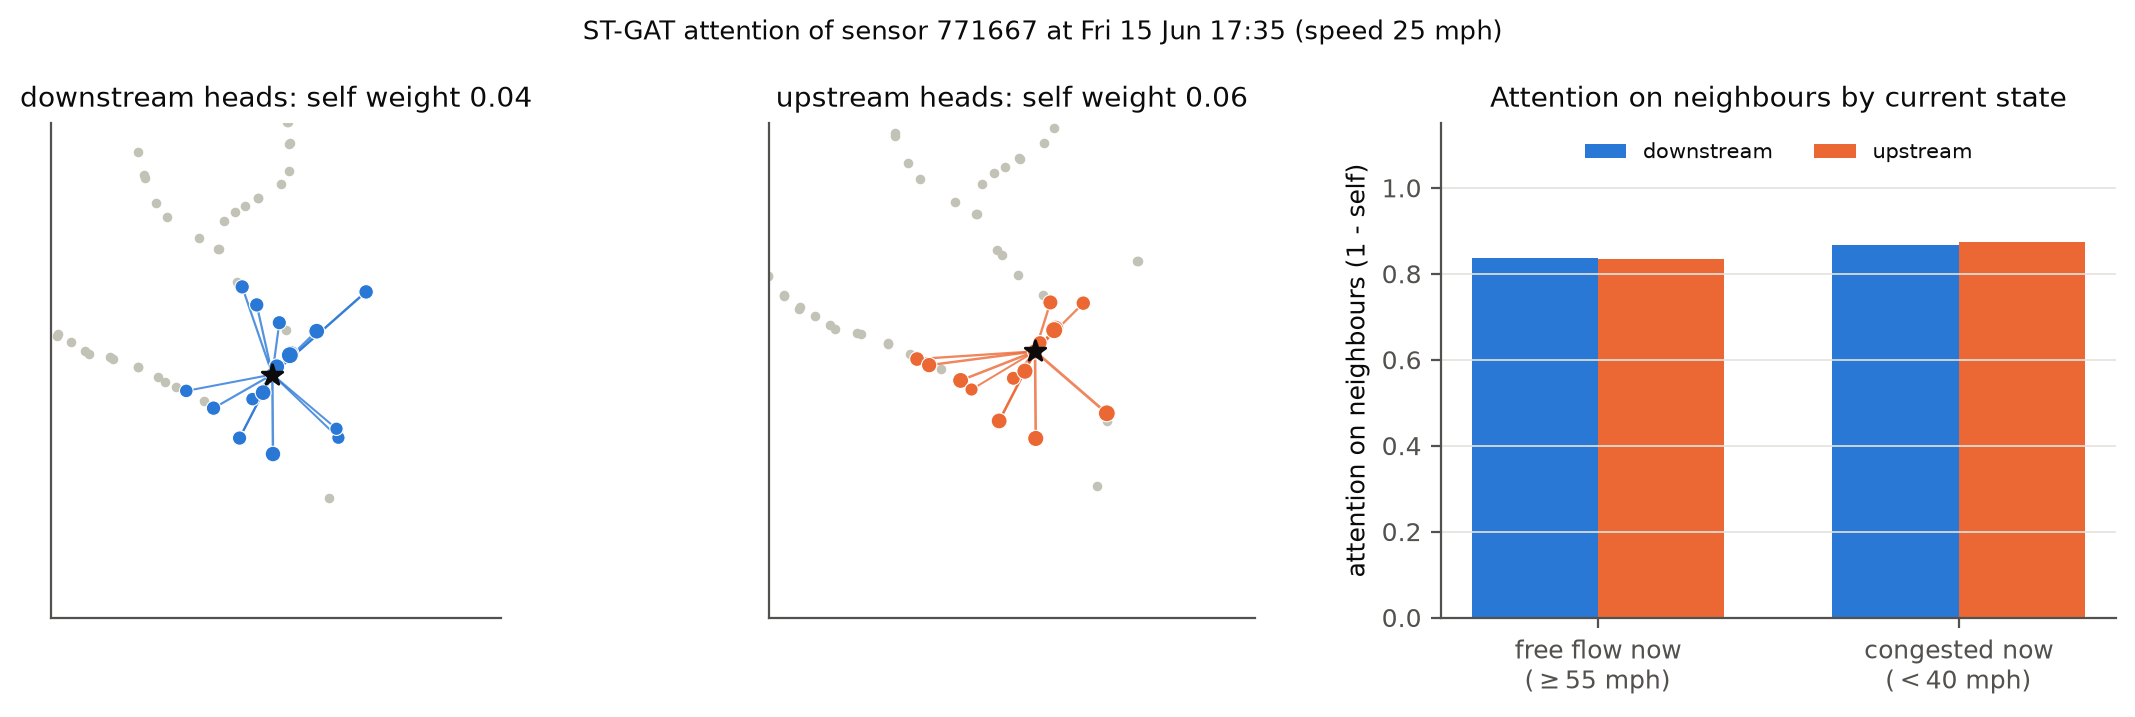
\includegraphics[width=\textwidth]{p2_attention.png}
\caption{Attention weights of one congested sensor (downstream and upstream heads) and the
average attention on neighbours for free-flowing and congested sensors.}
\label{fig:attn}
\end{figure*}

% ---------------------------------------------------------------- 5
\section{Model 3: Hybrid XGBoost and Graph Attention}
\subsection{Idea}
XGBoost per segment is good at the usual pattern and recent trend of its own segment, while
ST-GAT can see the neighbours. The hybrid combines them: it keeps the XGBoost forecast and lets
a graph attention network learn only a correction,
\begin{equation}
\hat y_i=\hat y_i^{\,\mathrm{XGB}}+g_\theta\big(X,\hat Y^{\mathrm{XGB}}\big)_i ,
\end{equation}
where $g_\theta$ receives the same input window as ST-GAT together with the XGBoost forecasts
of all sensors. This is similar to the classical approach of fitting a neural network to the
errors of another model~\cite{zhang2003hybrid}.

\begin{figure}[t]
\centering
\resizebox{\columnwidth}{!}{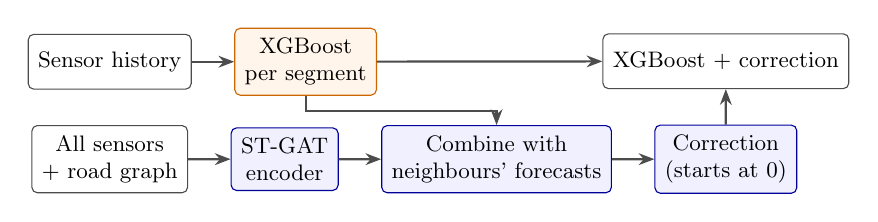
\begin{tikzpicture}[node distance=5mm and 6mm, scale=0.9, transform shape]
\node[box] (x) {Sensor history};
\node[ml, right=of x] (xgb) {XGBoost\\per segment};
\node[box, below=of x] (g) {All sensors\\+ road graph};
\node[dl, right=of g] (st) {ST-GAT\\encoder};
\node[dl, right=of st] (fuse) {Combine with\\neighbours' forecasts};
\node[dl, right=of fuse] (head) {Correction\\(starts at 0)};
\node[box, above=5mm of head] (sum) {XGBoost + correction};
\draw[arr] (x) -- (xgb); \draw[arr] (g) -- (st); \draw[arr] (st) -- (fuse); \draw[arr] (fuse) -- (head);
\draw[arr] (xgb) -- (sum);
\draw[arr] (xgb.south) |- ([yshift=2mm]fuse.north) -- (fuse.north);
\draw[arr] (head) -- (sum);
\end{tikzpicture}}
\caption{The hybrid model.}
\label{fig:hybrid}
\end{figure}

The network uses the ST-GAT encoder, adds a layer that embeds the XGBoost forecasts, and one
more graph attention layer so that a sensor can look at the XGBoost forecasts of its
neighbours (Fig.~\ref{fig:hybrid}). The last layer is initialised to zero, so before training
the hybrid gives exactly the XGBoost forecast. It has 181,052 parameters.

\subsection{Avoiding leakage with cross-fitting}
If the correction network were trained on XGBoost forecasts for the same windows XGBoost was
trained on, it would see errors that are much smaller than at test time (2.69\,mph instead of
2.99\,mph on the training data). It would then learn to trust XGBoost too much. We therefore
split the training period into five consecutive blocks. For each block we train XGBoost on the
other four, leaving out the 23 time steps around the block so that no window overlaps it, and
use that model to forecast the block~\cite{wolpert1992stacking,bergmeir2012cv}. The
validation and test windows get forecasts from the XGBoost model trained on all training
data.

\subsection{Training and corrections}
The correction network is trained in the same way as ST-GAT. It starts from the XGBoost
forecast, reaches its best validation MAE of 2.87\,mph and then levels off after about 25
epochs while the training error keeps falling, which means it starts to overfit. On the test
set the average correction is 0.95\,mph. It is larger in peak hours (1.71\,mph) than off-peak
(0.70\,mph) and largest when the traffic turns out to be congested (3.27\,mph), so the
network mostly changes the forecast where congestion spreads between segments.

% ---------------------------------------------------------------- 6
\section{Results}
\subsection{Accuracy}
Table~\ref{tab:main} and Fig.~\ref{fig:horizon} compare the three models on the test set.
ST-GAT lowers the average MAE of the per-segment models from 3.20 to 3.04\,mph (5\,\%), and the
hybrid to 3.06\,mph. The hybrid is the most accurate up to 20 minutes ahead, and ST-GAT from 25
minutes on. The Diebold--Mariano test shows that both network models are better than XGBoost
per segment at 15, 30 and 60 minutes ($p<0.001$). At 60 minutes ST-GAT (3.47\,mph) is also
below the results published for DCRNN (3.60)~\cite{li2018dcrnn} and Graph WaveNet
(3.53)~\cite{wu2019gwnet} on the same data.

\begin{table*}[t]
\centering
\caption{Test results (lower is better). MAE and RMSE in mph, MAPE in \%.}
\label{tab:main}
\small
\begin{tabular}{lccccccccc}
\toprule
 & \multicolumn{3}{c}{15 min} & \multicolumn{3}{c}{30 min} & \multicolumn{3}{c}{60 min} \\
\cmidrule(lr){2-4}\cmidrule(lr){5-7}\cmidrule(lr){8-10}
Model & MAE & RMSE & MAPE & MAE & RMSE & MAPE & MAE & RMSE & MAPE \\
\midrule
XGBoost per segment & 2.89 & 5.67 & 8.14 & 3.26 & 6.62 & 9.71 & 3.64 & 7.50 & 11.35 \\
ST-GAT & 2.74 & \textbf{5.23} & 7.45 & \textbf{3.08} & \textbf{6.26} & 8.88 & \textbf{3.47} & \textbf{7.30} & 10.58 \\
Hybrid & \textbf{2.72} & \textbf{5.23} & \textbf{7.22} & 3.09 & 6.29 & \textbf{8.77} & 3.52 & 7.35 & \textbf{10.57} \\
\bottomrule
\end{tabular}
\end{table*}

\begin{figure*}[t]
\centering
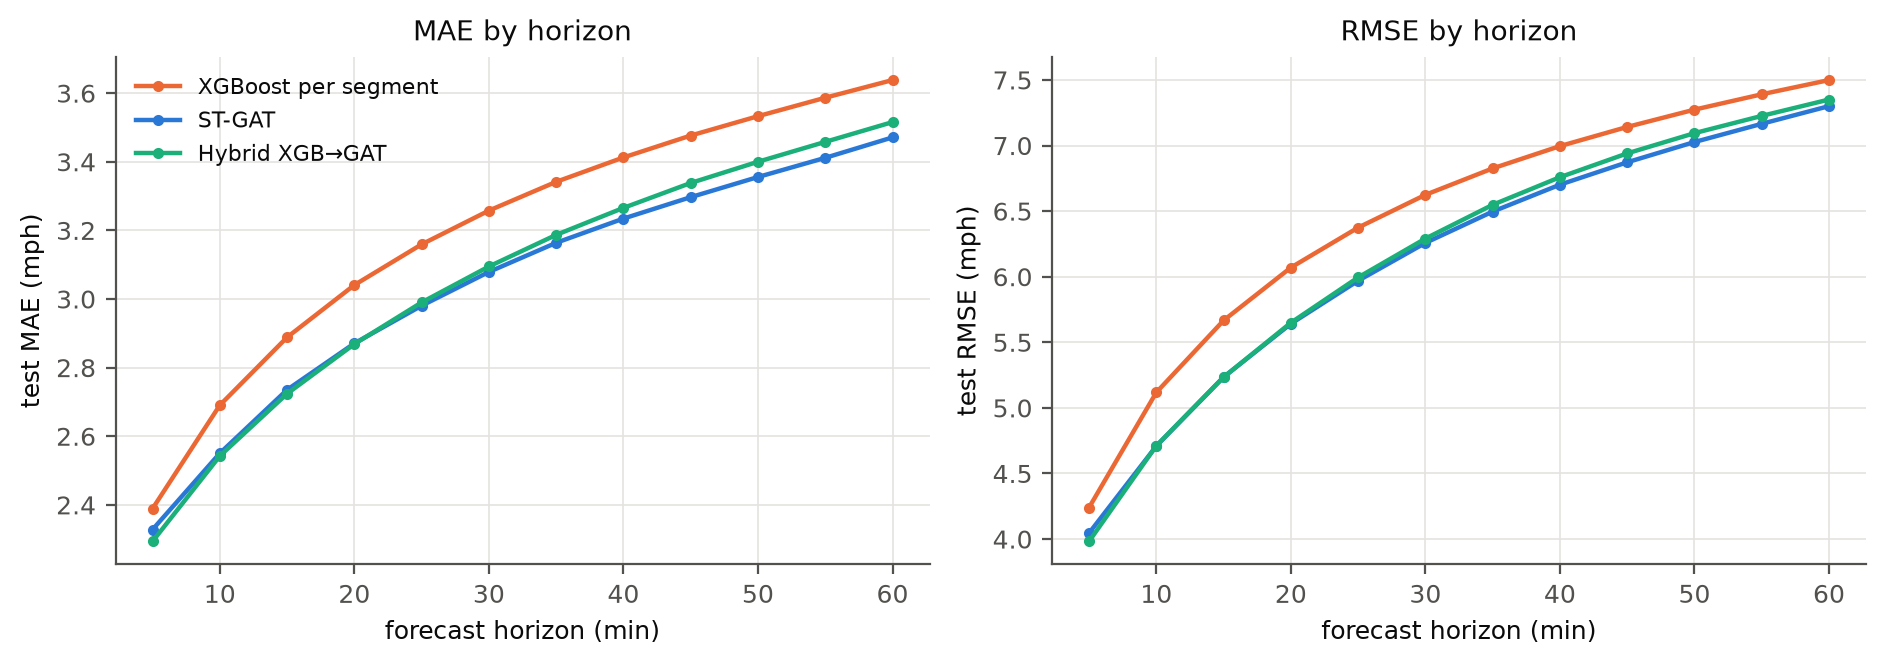
\includegraphics[width=0.9\textwidth]{p2_horizon_three.png}
\caption{Test MAE and RMSE at all 12 horizons.}
\label{fig:horizon}
\end{figure*}

\subsection{Peak hours, congestion and missing readings}
The network models help most when traffic is hard to predict (Table~\ref{tab:peak}). At 60
minutes, ST-GAT lowers the error in peak hours from 5.19 to 4.88\,mph (6\,\%) but off-peak only
from 3.07 to 2.96\,mph. On congested readings the error drops by more than 1\,mph. When a
sensor's latest reading is missing, the 60-minute error of ST-GAT rises by 28\,\%, compared
with 32\,\% for XGBoost per segment and 34\,\% for the hybrid.

\begin{table}[t]
\centering
\caption{Test MAE (mph) in peak hours, off-peak and on congested readings ($<$40\,mph).}
\label{tab:peak}
\footnotesize
\setlength{\tabcolsep}{3pt}
\begin{tabular}{lccccccc}
\toprule
 & \multicolumn{3}{c}{Peak} & \multicolumn{3}{c}{Off-peak} & Cong. \\
\cmidrule(lr){2-4}\cmidrule(lr){5-7}\cmidrule(lr){8-8}
Model & 15 & 30 & 60 & 15 & 30 & 60 & 60 \\
\midrule
XGBoost & 3.82 & 4.49 & 5.19 & 2.54 & 2.81 & 3.07 & 11.79 \\
ST-GAT & 3.57 & 4.19 & \textbf{4.88} & \textbf{2.43} & \textbf{2.67} & \textbf{2.96} & \textbf{10.66} \\
Hybrid & \textbf{3.50} & \textbf{4.16} & 4.94 & 2.44 & 2.70 & 2.99 & 10.74 \\
\bottomrule
\end{tabular}
\end{table}

Figure~\ref{fig:map} shows one evening rush hour. The per-segment models underestimate how far
the slowdown spreads along the main corridor, while the two network models get closer to the
observed speeds.

\begin{figure*}[t]
\centering
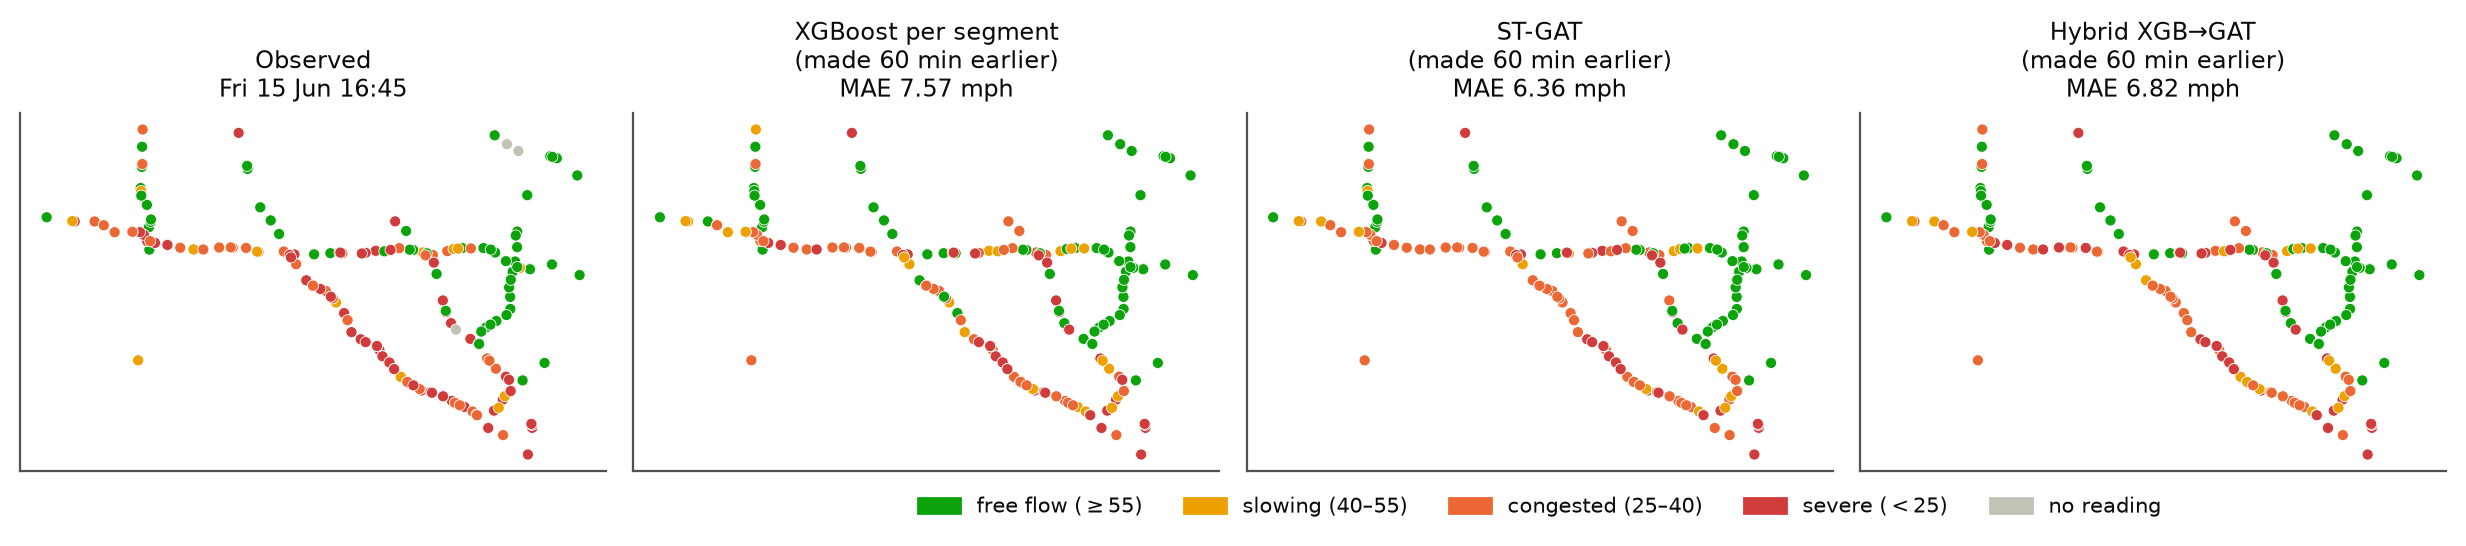
\includegraphics[width=\textwidth]{p2_congestion_map.png}
\caption{Observed speeds during an evening peak and the forecasts made 60 minutes earlier.}
\label{fig:map}
\end{figure*}

Over the whole test period, the hybrid is more accurate than XGBoost per segment at 79\,\% of
the sensors at 60 minutes ahead (Fig.~\ref{fig:improve}). The largest improvements are on the
long corridor that is congested most often.

\begin{figure}[t]
\centering
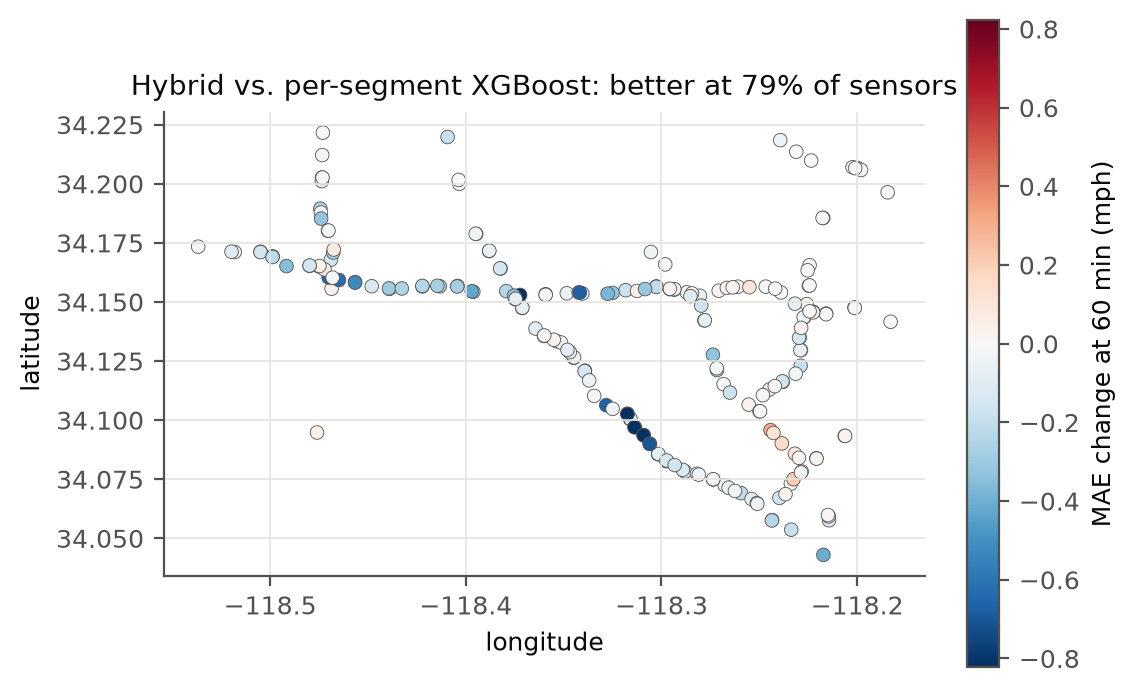
\includegraphics[width=\columnwidth]{p2_improvement_map.png}
\caption{Change in 60-minute MAE for each sensor, hybrid minus XGBoost per segment (blue means
the hybrid is better).}
\label{fig:improve}
\end{figure}

\subsection{Ablation studies}
To see which parts of the models matter, we trained variants with one part removed, all
with the same budget of 12 epochs and the same random seed (Table~\ref{tab:abl}). For ST-GAT,
feeding missing readings as 0\,mph hurts the most, and removing the graph layers brings the
model back to the level of XGBoost per segment (3.20\,mph), which shows that the gain comes
from using the road network. Letting attention look at all sensor pairs instead of road
neighbours is worse, and plain averaging of the neighbours is only slightly worse than
attention. For the hybrid, both the graph and cross-fitting are needed. With this equal budget
the hybrid is better than ST-GAT at every horizon (3.05 against 3.08\,mph); with longer
training ST-GAT catches up because the hybrid starts to overfit.

\begin{table}[t]
\centering
\caption{Ablations: average test MAE (mph), each variant trained for 12 epochs.}
\label{tab:abl}
\footnotesize
\begin{tabular}{lc}
\toprule
Variant & MAE \\
\midrule
\multicolumn{2}{l}{\textit{ST-GAT}} \\
Full model & \textbf{3.08} \\
Averaging instead of attention & 3.10 \\
Attention over all sensor pairs & 3.14 \\
Without graph layers & 3.20 \\
Missing readings fed as 0\,mph & 3.23 \\
\midrule
\multicolumn{2}{l}{\textit{Hybrid}} \\
Full hybrid & \textbf{3.05} \\
XGBoost forecast as input only & 3.07 \\
Without cross-fitting & 3.14 \\
Correction without graph & 3.16 \\
Linear correction & 3.19 \\
\bottomrule
\end{tabular}
\end{table}

\subsection{Training curves}
Figure~\ref{fig:curves} shows the training and validation error of ST-GAT and the hybrid.
ST-GAT keeps improving slowly until the end of training. The hybrid starts close to the
XGBoost forecast, improves quickly in the first epochs and then levels off, while its training
error keeps going down. This is why the hybrid is the better model after a short training run
and ST-GAT catches up when both are trained for 40 epochs.

\begin{figure}[t]
\centering
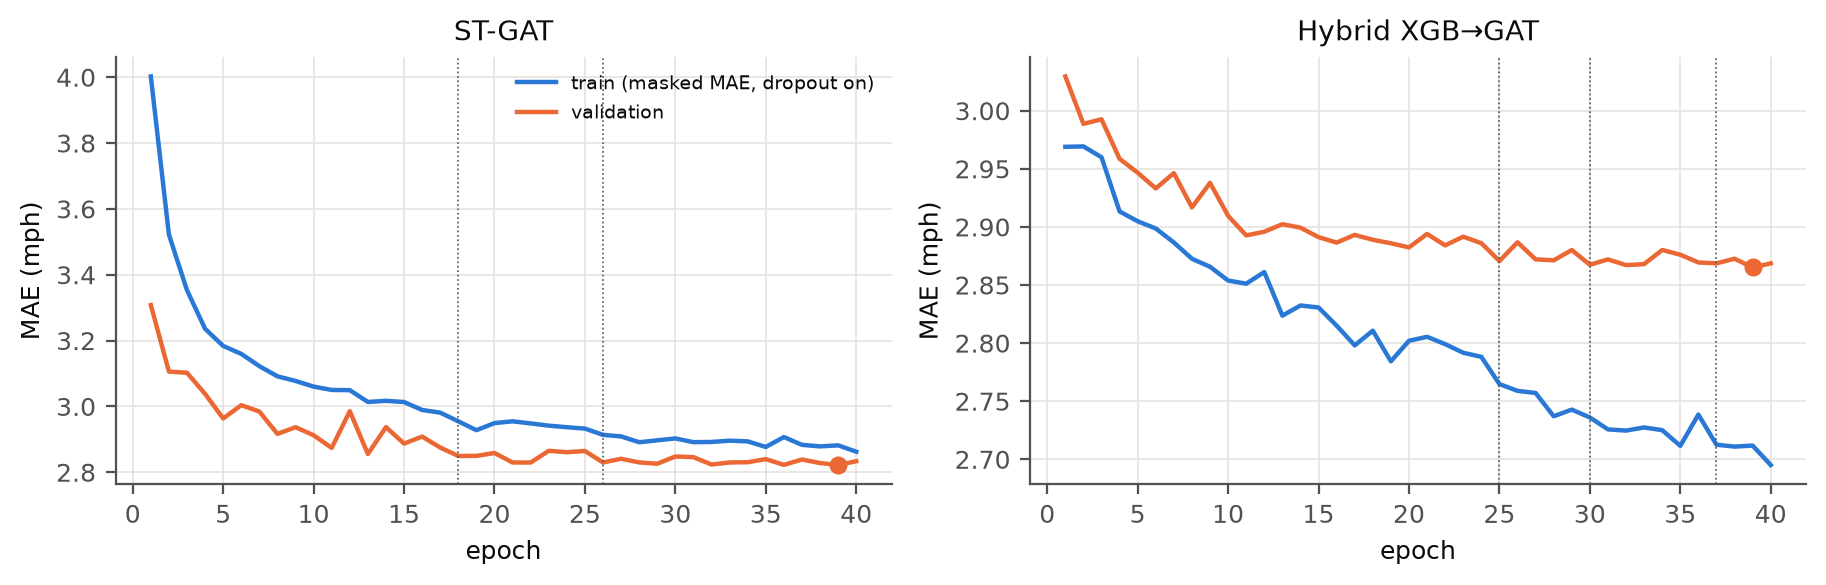
\includegraphics[width=\columnwidth]{p2_learning_curves.png}
\caption{Training and validation MAE per epoch (dots: best epoch; dotted lines: learning-rate
halvings).}
\label{fig:curves}
\end{figure}

\subsection{Simulated signal control}
As a simple use case we replayed the test period offline. At every 5-minute step, a controller
at each sensor switches to a congestion plan if the forecast for 15 minutes ahead is below
40\,mph. We count how many of the 6,554 congestion onsets were anticipated, meaning the plan
was already on in the 30 minutes before the speed dropped (Table~\ref{tab:signal}). A
controller that only reacts to the current speed cannot anticipate any onset. With forecasts,
the plan is switched on in time for 20\,\% (XGBoost), 30\,\% (ST-GAT) and 36\,\% (hybrid) of the
onsets, with fewer false activations. METR-LA has no signal timings or turning counts, so this
only measures when a decision would be made, not how much delay it would save.

\begin{table}[t]
\centering
\caption{Offline signal-plan simulation on the test period: onsets anticipated, false
activations, and plan switches per sensor-day.}
\label{tab:signal}
\footnotesize
\begin{tabular}{lccc}
\toprule
Policy & Anticip.\ (\%) & False (\%) & Switches \\
\midrule
React to current speed & 0.0 & 10.6 & 6.6 \\
XGBoost per segment & 19.8 & 7.7 & 4.1 \\
ST-GAT & 30.1 & 7.7 & 3.4 \\
Hybrid & 35.7 & 6.0 & 3.8 \\
\bottomrule
\end{tabular}
\end{table}

% ---------------------------------------------------------------- 7
\section{Conclusion}
Separate models for each road segment leave useful information unused: their errors are
correlated with what is happening on neighbouring roads. A graph attention network that uses
the road graph lowers the forecast error by about 5\,\% overall and 6\,\% in rush hour at 60
minutes, and the improvement is statistically significant at every horizon. The hybrid model
shows that XGBoost and graph attention can be combined well when the XGBoost forecasts used for
training are cross-fitted; it gives the best forecasts up to 20 minutes ahead and learns
fastest. The ablations show that using the road graph and treating missing readings correctly
matter most.

The project has some limitations. Each model was trained once with one random seed on a
laptop, the dataset has speed only and covers four months, and the signal experiment is an
offline replay. Possible next steps are training with several seeds, adding flow and occupancy
from the PeMS data, using GATv2~\cite{brody2022gatv2} attention, and testing the forecasts in a
traffic simulator such as SUMO~\cite{krajzewicz2012sumo}.

\bibliographystyle{IEEEtran}
\bibliography{../report/refs}

\end{document}
